\documentclass [12pt, a4paper]{article}\usepackage[]{graphicx}\usepackage[]{color}
%% maxwidth is the original width if it is less than linewidth
%% otherwise use linewidth (to make sure the graphics do not exceed the margin)
\makeatletter
\def\maxwidth{ %
  \ifdim\Gin@nat@width>\linewidth
    \linewidth
  \else
    \Gin@nat@width
  \fi
}
\makeatother

\definecolor{fgcolor}{rgb}{0.345, 0.345, 0.345}
\newcommand{\hlnum}[1]{\textcolor[rgb]{0.686,0.059,0.569}{#1}}%
\newcommand{\hlstr}[1]{\textcolor[rgb]{0.192,0.494,0.8}{#1}}%
\newcommand{\hlcom}[1]{\textcolor[rgb]{0.678,0.584,0.686}{\textit{#1}}}%
\newcommand{\hlopt}[1]{\textcolor[rgb]{0,0,0}{#1}}%
\newcommand{\hlstd}[1]{\textcolor[rgb]{0.345,0.345,0.345}{#1}}%
\newcommand{\hlkwa}[1]{\textcolor[rgb]{0.161,0.373,0.58}{\textbf{#1}}}%
\newcommand{\hlkwb}[1]{\textcolor[rgb]{0.69,0.353,0.396}{#1}}%
\newcommand{\hlkwc}[1]{\textcolor[rgb]{0.333,0.667,0.333}{#1}}%
\newcommand{\hlkwd}[1]{\textcolor[rgb]{0.737,0.353,0.396}{\textbf{#1}}}%
\let\hlipl\hlkwb

\usepackage{framed}
\makeatletter
\newenvironment{kframe}{%
 \def\at@end@of@kframe{}%
 \ifinner\ifhmode%
  \def\at@end@of@kframe{\end{minipage}}%
  \begin{minipage}{\columnwidth}%
 \fi\fi%
 \def\FrameCommand##1{\hskip\@totalleftmargin \hskip-\fboxsep
 \colorbox{shadecolor}{##1}\hskip-\fboxsep
     % There is no \\@totalrightmargin, so:
     \hskip-\linewidth \hskip-\@totalleftmargin \hskip\columnwidth}%
 \MakeFramed {\advance\hsize-\width
   \@totalleftmargin\z@ \linewidth\hsize
   \@setminipage}}%
 {\par\unskip\endMakeFramed%
 \at@end@of@kframe}
\makeatother

\definecolor{shadecolor}{rgb}{.97, .97, .97}
\definecolor{messagecolor}{rgb}{0, 0, 0}
\definecolor{warningcolor}{rgb}{1, 0, 1}
\definecolor{errorcolor}{rgb}{1, 0, 0}
\newenvironment{knitrout}{}{} % an empty environment to be redefined in TeX

\usepackage{alltt}

\usepackage{amsmath,amsfonts,amssymb,amsthm,mathtools}
\usepackage{etoolbox}

%%Шрифты%%
\usepackage{fontspec}         % пакет для подгрузки шрифтов
\setmainfont{Arial}   % задаёт основной шрифт документа

% Чтобы пропечатывались длинные тире, непрерывные пробелы и тп
\defaultfontfeatures{Mapping=tex-text}

\newfontfamily{\cyrillicfonttt}{Arial}
\newfontfamily{\cyrillicfont}{Arial}
\newfontfamily{\cyrillicfontsf}{Arial}

\usepackage{unicode-math}     % пакет для установки математического шрифта
\setmathfont{Asana Math}      % шрифт для математики

\usepackage{polyglossia}      % Пакет, который позволяет подгружать русские буквы
\setdefaultlanguage{russian}  % Основной язык документа
\setotherlanguage{english}    % Второстепенный язык документа
% Разные мелочи для русского языка из пакета babel
\setkeys{russian}{babelshorthands=true}

\usepackage{indentfirst} % установка отступа в первом абзаце главы!!!
\usepackage{booktabs} 
\usepackage{float}

\usepackage[paper=a4paper,top=13.5mm, bottom=13.5mm, left=16.5mm, right=13.5mm, includefoot]{geometry}

\title{Отчёт о расчёте VaR по ПАО "Альфа-Банк"}
%А где ещё Винни работать, кроме как Альфа-Банка?! В Сбере, я думаю, не всё так просто.
\author{Винни-Пух}
\date{\today}
\IfFileExists{upquote.sty}{\usepackage{upquote}}{}
\begin{document}

\title{\vspace{10cm} Отчёт о расчёте VaR по ПАО "Альфа-Банк"}
%А где ещё Винни работать, кроме как в Альфа-Банке?! В Сбере, я думаю, не всё так просто, чтобы народ полдня прохлаждался.

\author{Винни-Пух}
\date{\today}

\maketitle

\thispagestyle{empty}

\newpage

\section{VaR}

 В данном отчёте расчитываются VaR. Делается это с помощью нормального распределения. Реалистичность расчётов проверяется с помощью теста Купика.
\vspace{3cm}


\begin{knitrout}
\definecolor{shadecolor}{rgb}{0.969, 0.969, 0.969}\color{fgcolor}

{\centering 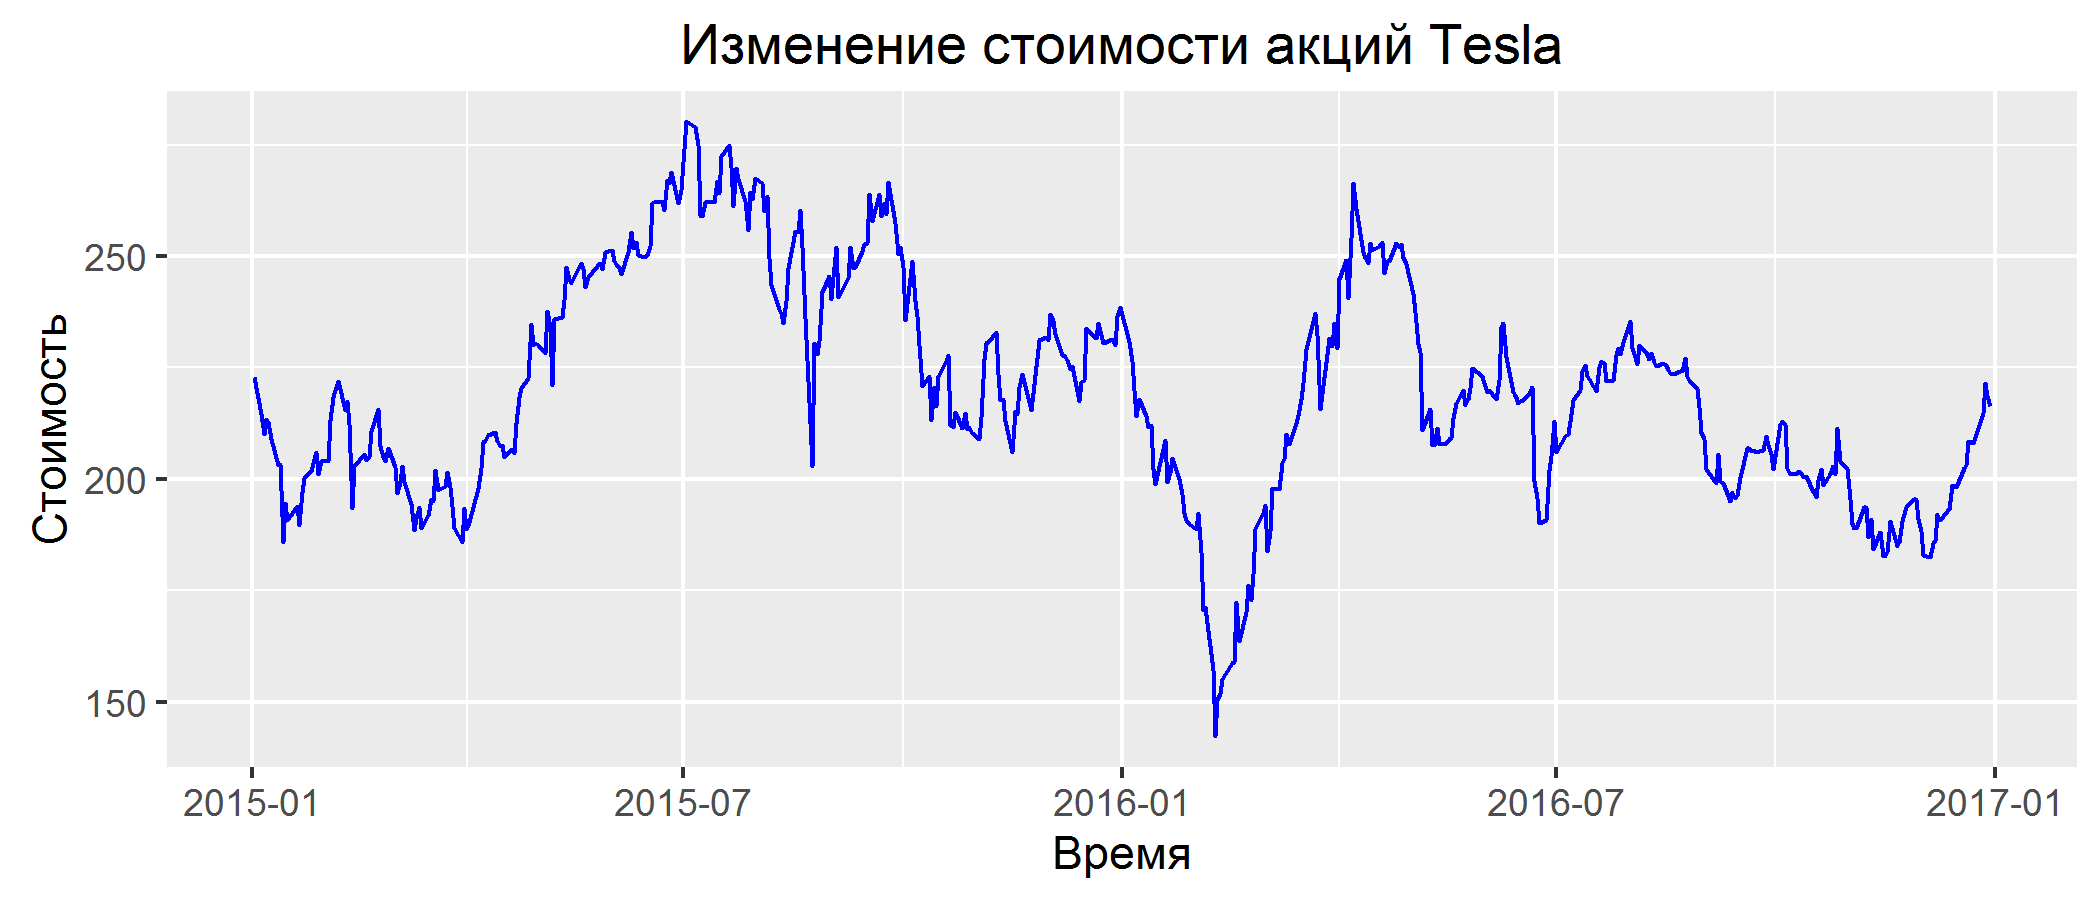
\includegraphics[width=\maxwidth]{figure/plot-1} 

}



\end{knitrout}
\vspace{2cm}
\begin{knitrout}
\definecolor{shadecolor}{rgb}{0.969, 0.969, 0.969}\color{fgcolor}

{\centering 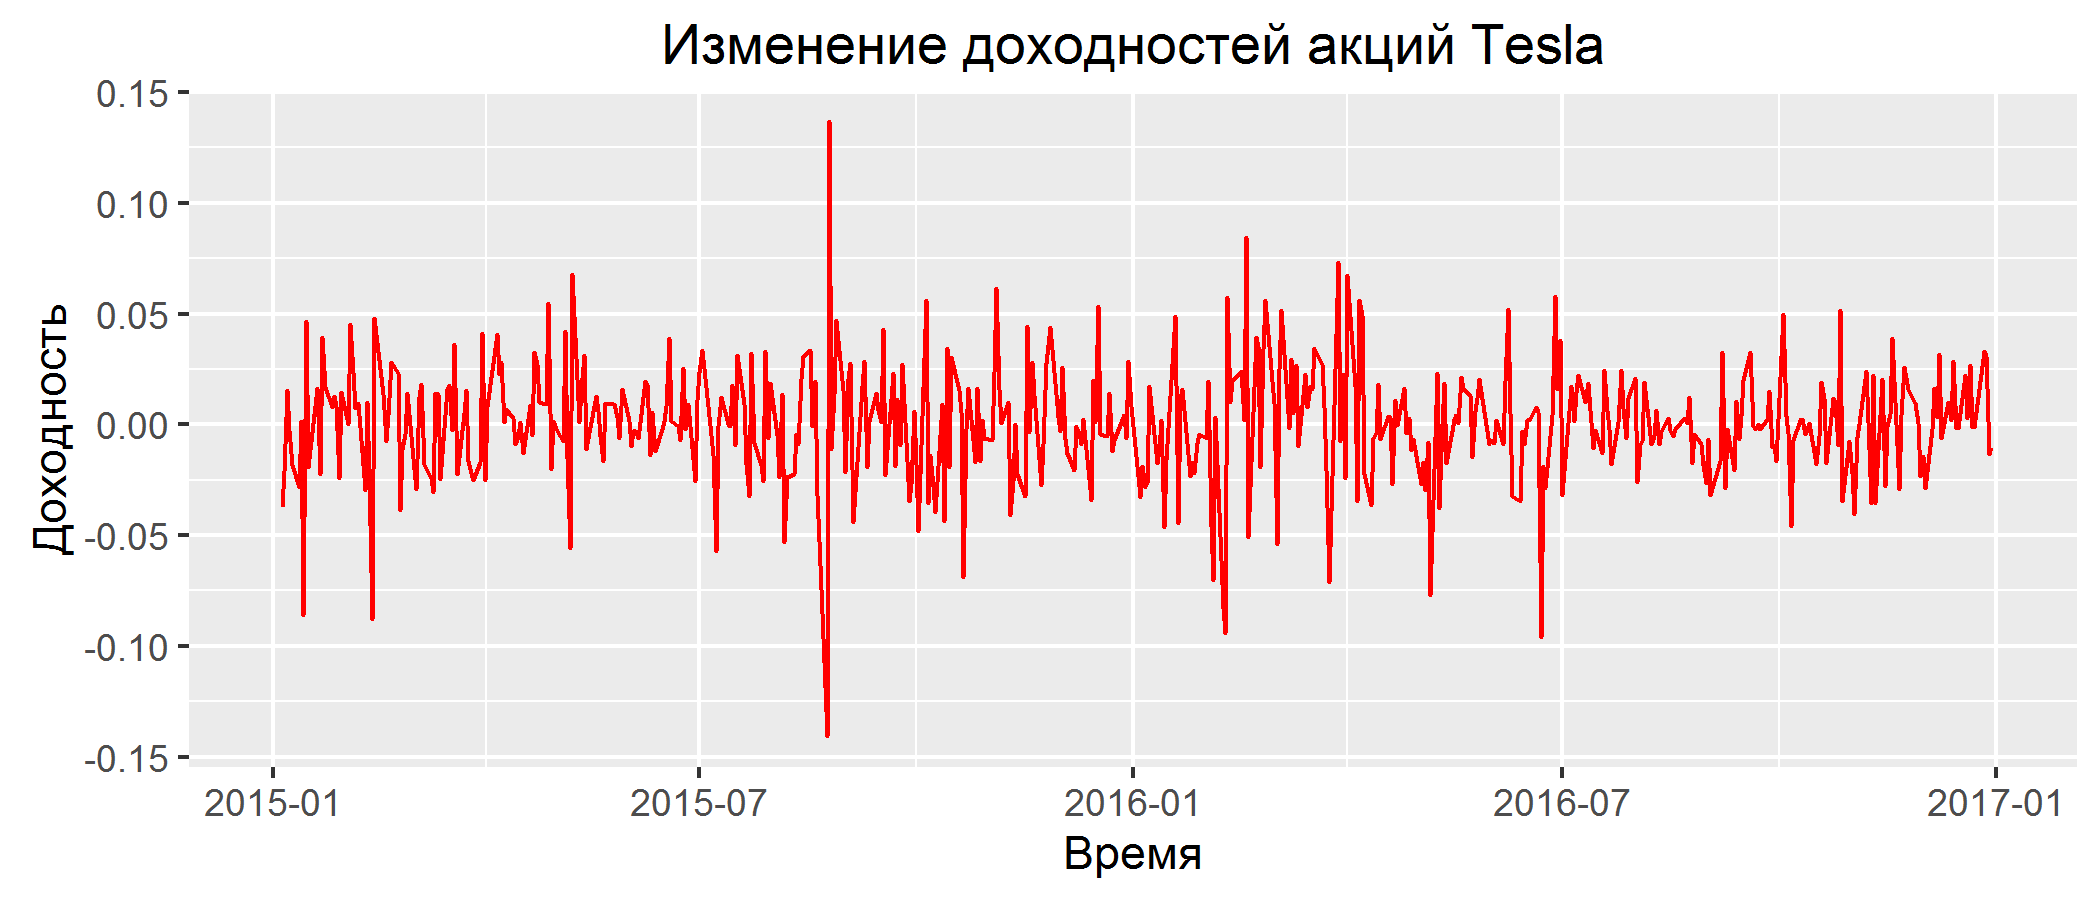
\includegraphics[width=\maxwidth]{figure/rate_of_return_plot-1} 

}



\end{knitrout}

\vfill
 \begin{center}
 \textbf {\Large VaR = -0.0438916}
 \end{center}
 
\clearpage
\section {Адекватность расчёта VaR}
 
 
\begin{knitrout}
\definecolor{shadecolor}{rgb}{0.969, 0.969, 0.969}\color{fgcolor}

{\centering 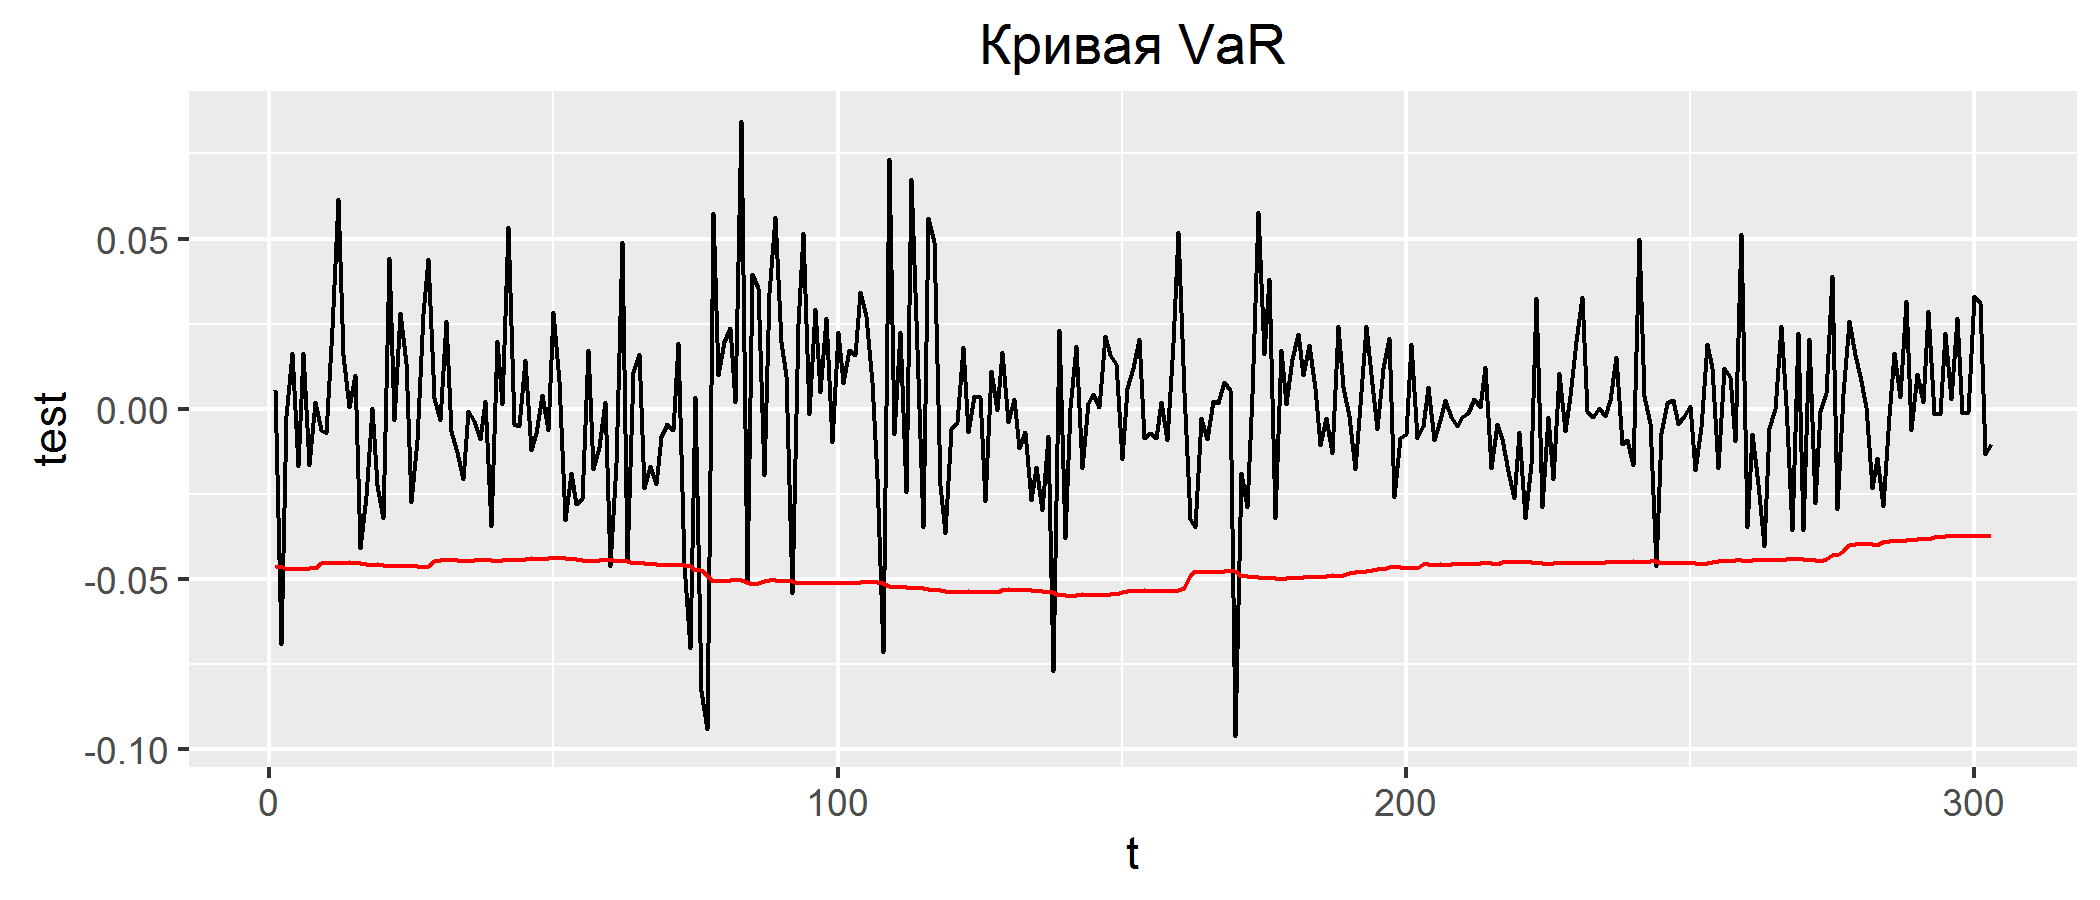
\includegraphics[width=\maxwidth]{figure/Var_curve-1} 

}



\end{knitrout}



$p-value$ для теста Купика равно 25.11 \%. \ifstrequal{good}{good}{Наш прогноз хороший, так как гипотеза о том, что число пробитий не превышает 5\%, не отвергается. Прогноз заверен Купиком!}{Наш прогноз плохой, так как гипотеза о том, что число пробитий не превышает 5\%, отвергается.}

\section{Проверка гипотезы единичного корня. Расширенный тест Дики-Фуллера}



\begin{table}[h!]
 \caption{Результаты теста}
 \begin{center}
  
\begin{tabular}{l|l}
\hline
parametr & value\\
\hline
statistic & -7.72\\
\hline
lag order & 7\\
\hline
alternative & stationary\\
\hline
p-value & 0.01\\
\hline
\end{tabular}


 \end{center}
\end{table}

\vfill

 \begin{flushright}
 \rule{5em}{0.5pt} Пятачок
 \end{flushright}
\end{document}
